\subsection{Le primitive nella modellazione UML}

Le primitive descritte nella Figura \ref{fig:rdy} vengono rappresentate anche nella modellazione del protocollo attraverso l'utilizzo dei diagrammi UML.\\
La primitiva $G_{concat}$ (concatenazione) appare nei diagrammi UML quando abbiamo più input in ingresso ad un oggetto con un singolo output, ad esempio viene utilizzata quando in un oggetto viene preparato un pacchetto, dati vari parametri in ingresso vengono concatenati prima di essere inoltrati.\\
Al contrario la primitiva $A_{concat}$ (deconcatenazione) appare quando abbiamo un singolo input e in uscita più output, come quando abbiamo in ingresso un pacchetto e dobbiamo ricavare qualche elemento da cui è composto.\\
\begin{figure}[h!] 
    \centering 
        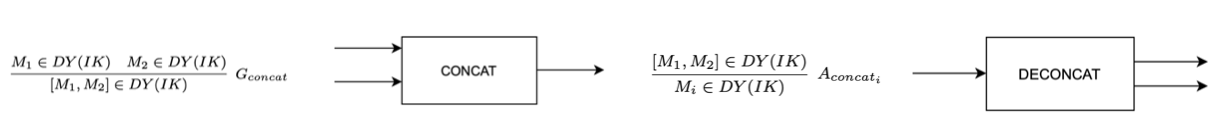
\includegraphics[width=\textwidth]{../img/1.png} 
        \caption{Concatenazione e deconcatenazione} 
\end{figure}\\
Nella modellazione UML gli oggetti di encryption e decryption sono considerati delle black box, questo perch\'e in caso di crittografia simmetrica corrispondono alle primitive $G_{critS}$ e $A_{critS}$ e in caso di crittografia asimmetrica corrispondono alle primitive $G_{crittA}$ e $A_{crittA}$ del modello Dolev-Yao.\\
\begin{figure}[h!] 
    \centering 
        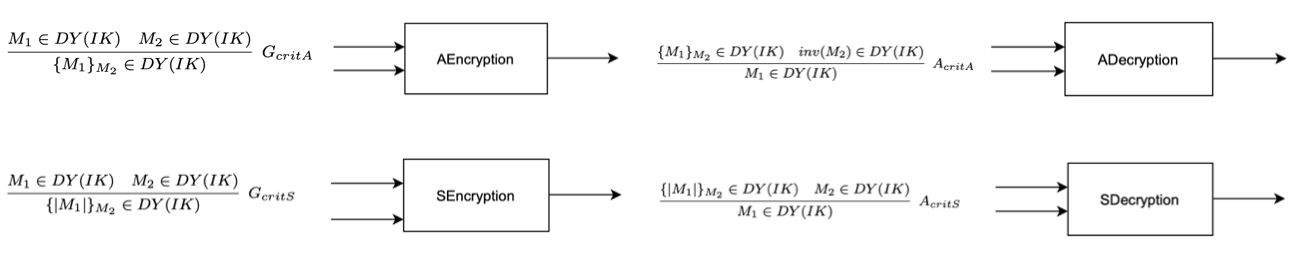
\includegraphics[width=\textwidth]{../img/2.png} 
        \caption{Encryption e decryption a chiave simmetrica e asimmetrica} 
\end{figure}\\
Nel caso in cui nel diagramma sia rappresentato un oggetto per la firma di un messaggio o per la verifica della firma, ancora una volta troviamo nel modello Dolev-Yao le primitive necessarie, ovvero la primitiva  $G_{crittA}$, la quale si occupa della firma di un messaggio prendendo come input la chiave privata e il messaggio, e la primitiva $A^{-1}_{crittA}$, la quale verifica la firma utilizzando la chiave pubblica.\\
\begin{figure}[h!] 
    \centering 
        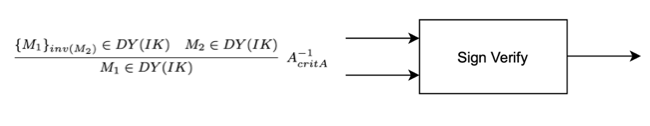
\includegraphics[width=0.6\textwidth]{../img/3.png} 
        \caption{Verifica della firma} 
\end{figure}\\
\begin{figure}[h!] 
    \centering 
        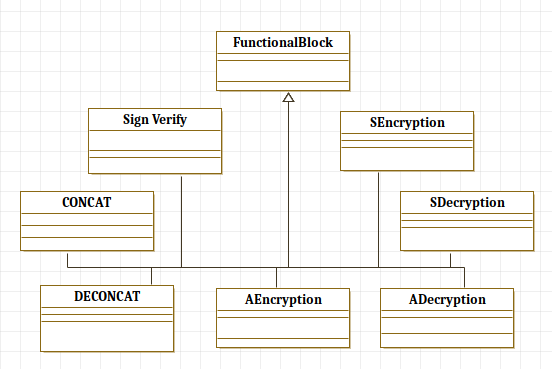
\includegraphics[width=0.8\textwidth]{../img/cd_1.png} 
        \caption{Diagramma delle classi delle primitive} 
\end{figure}\\
